%Modul 1


%Overskrift
\begin{center}
\Huge
Intro til matematik i gymnasiet
\end{center}
\section*{Matematik som videnskab}
\stepcounter{section}


I den rene matematik arbejder vi på at beskrive og analysere matematiske objekter og deres indbyrdes sammenhæng. Vi vil typisk konstruere definitioner, og så prøve at bevise resultater om disse definitioner. Sådanne resultater kaldes tit for sætninger. Som eksempel kan vi være interesseret i heltallenes egenskaber.
\begin{exa}\label{exa:exa1}
Vi husker på, at et primtal er et heltal, der kun har sig selv og $1$ som faktor. Det er altså et tal, ingen andre tal går op i. Små eksempler på disse kunne være $2,3,5,7,11$ og $13$. Det er ikke umiddelbart klart, om der kommer et punkt, hvor tal er så store, at der ikke er flere primtal. Vi vil bevise, at dette ikke er tilfældet. Vi opstiller derfor en sætning, som vi så vil bevise. Før vi kan bevise dette, skal vi dog bruge et hjælperesultat (nogle gange kaldt et lemma).
\begin{setn}\label{setn:divlemma}
Hvis $d$ går op i $a_1$ og $d$ går op i $a_2$, så går $d$ op i $a_1-a_2$.
\end{setn}
\begin{proof}
Antag, at $d$ går op i både $a_1$ og $a_2$. Det betyder, at $a_1 = db_1$ og $a_2=db_2$ for to tal $b_1,b_2$. Dette medfører så, at  
\[
a_1-a_2 = db_1-db_2=d(b_1-b_2),
\]
og $d$ går derfor op i $a_1-a_2$.
\end{proof}
\begin{setn}
Der er uendeligt mange primtal. 
\end{setn}
\begin{proof}
Antag, at der er endeligt mange primtal, som vi kan opskrive
\begin{align*}
p_1,p_2,\hdots,p_n.
\end{align*}
Vi lader $P = p_1p_2\cdots p_n$ og $Q = P+1$.  

Der er to tilfælde:
\begin{enumerate}[label=\roman*)]
 \item$Q$ er selv et primtal som vi kan tilføje til listen $p_1,\hdots,p_n$, eller
 \item $Q$ er ikke et primtal og der findes et primtal $p$, der går op i $Q$. Hvis $p$ er en del af listen $p_1,\hdots,p_n$, så går $p$ op i $P=p_1p_2\cdots p_n$. Derfor går $p$ både op i $P$ og $Q$, men i følge Sætning \ref{setn:divlemma}, så går $p$ også op i $Q-P = (P+1)-P = 1$, så derfor kan $p$ ikke have været i listen $p_1,\hdots,p_n$, og vi kan altså tilføje $p$ til listen. 
\end{enumerate}
\end{proof}
\end{exa}
\begin{exa}\label{exa:exa2}
Et meget berømt problem i talteori går ud på at beskrive for hvilke naturlige tal ($0,1,2,\hdots$) $n$ ligningen 
\begin{align*}
a^n+b^n=c^n
\end{align*}
har løsninger, når $a,b,c$ er heltal. Hvis $n=2$, så har vi uendeligt mange løsninger. Dette er blot Pythagoras' sætning. I tilfældet $n>2$, så findes der ingen løsninger, og dette kaldes Fermats sidste sætning, men han gav aldrig selv et bevis (selvom han påstod det). Vi opskriver også dette som en sætning:
\begin{setn}
For heltal $n>2$ har ligningen 
\begin{align*}
a^n+b^n = c^n 
\end{align*}
ingen heltalsløsninger.
\end{setn}
\begin{proof}
Dette overlades til læseren
\end{proof}
\end{exa}
\subsection*{Eksempler på objekter samt lidt notation}
En af de simpleste matematiske objekter, vi kan støde på er mængder. Vi vil ikke give en stringent definition af, hvad en mængde er, men vi vil tænke på en mængde som en samling af elementer. Elementerne kan være alt, hvad hjertet begærer, men elementerne i de mængder, vi skal arbejde med vil oftest være tal. 
\begin{exa}
Vigtige eksempler på mængder er de naturlige tal $\mathbb{N} = \{0,1,2,\hdots\}$, de hele tal $\mathbb{Z} = \{\hdots,-2,-1,0,1,2\hdots\}$, de rationale tal $\mathbb{Q}$, der er tal, der kan skrives som en brøk af to heltal og de reelle tal $\mathbb{R}$, der er alle de rationale tal samt alle de tal, der "ligger mellem" de rationale tal (de irrationale tal). Vi kan beskrive deres indbyrdes inklusion ved et såkaldt Venn-diagram som set på Fig. \ref{fig:venn}.
\begin{figure}[H]
\centering
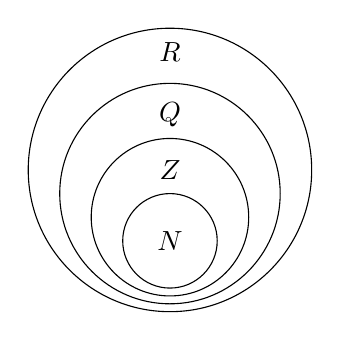
\begin{tikzpicture}
\draw (0.0,0.0) circle (0.6);
\draw (0.0,0.3) circle (1);
\draw (0.0,0.6) circle (1.4);
\draw (0.0,0.9) circle (1.8);
\node at (0,0) {$\mathbb{N}$};
\node at (0,0.9) {$\mathbb{Z}$};
\node at (0,1.6) {$\mathbb{Q}$};
\node at (0,2.4) {$\mathbb{R}$};
\end{tikzpicture}
\caption{Inklusionsforhold mellem $\mathbb{N},\mathbb{Z},\mathbb{Q}$ og $\mathbb{R}$.}
\label{fig:venn}
\end{figure}
\end{exa}
Den sidste vigtige mængde vi vil introducere er den tomme mængde $\emptyset$, der er mængden uden nogen elementer.


Hvis en mængde $A$ er indeholdt i en mængde $B$ skriver vi $A\subseteq B$. Hvis to mængder er ens, vil de være indeholdt i hinanden. Hvis $A$ er indeholdt i $B$, og det er vigtigt at understrege, at $A \neq B$, skriver vi $A\subsetneq B$. Af Fig. \ref{fig:venn} har vi, at $\mathbb{N} \subseteq \mathbb{Z} \subseteq \mathbb{Q} \subseteq \mathbb{R}$.

Hvis vi vil notere, at et element $a$ kommer fra en mængde $A$, bruger vi symbolet $\in$; altså $a\in A$
\subsubsection*{Mængdebygger-notation}
Når vi vil notere hvilke elementer, en mængde indeholder, kan vi bruge mængdebygger-notation. Hvis vi har få elementer, vil vi blot opremse elementerne som i følgende eksempel: $A = \{1,2,4,6,7\}$. Vi kan også bruge udeladelsesprikker/ellipse som når vi opskriver de naturlige tal $\mathbb{N} = \{0,1,2,\hdots\}$. Til slut kan vi bruge mængdebygger-notation, der består af en grundmængde og mindst én betingelse:
\[
A = \left\{ \textit{Grundmængde}\ \middle| \  \textit{Betingelse} \right\}.
\]
Dette er lettere at forstå gennem en række eksempler.
\begin{exa} \label{exa:setbuilder}
Vi kan beskrive de rationale tal med mængdebyggernotation som 
\[
\mathbb{Q} = \left\{\frac{a}{b} \in \mathbb{R}\ \middle| \ a,b\in \mathbb{Z}, b\neq 0 \right\},
\]
vi kan beskrive de naturlige tal som 
\[
\mathbb{N} = \left\{n\in \mathbb{Z} \ \middle| \ n\geq 0 \right\}
\]
og vi kan betegne mængden af lige tal $L$ som
\[
L = \left\{a \in \mathbb{Z} \ \middle| \  \textnormal{der findes }n\in \mathbb{Z} \textnormal{ så }a=2n \right\}.
\]
\end{exa}


\section*{Matematik som værktøj}
\stepcounter{section}
I gymnasiet (og specielt på B-niveau) vil vi hovedsagligt stifte bekendtskab med matematik som værktøj til at beskrive, modellere og analysere andre videnskaber. I skulle gerne have set flere eksempler på dette i jeres grundforløb, men vi vil også se på en række eksempler her. 
\begin{exa}
Vi forestiller os en situation, hvor en bakteriekoloni er i et medie, hvor kolonien har ubegrænset plads og næringsstof. Vi antager, at hverenkelt bakterie deler sig en gang per time under disse forhold. En enkelt bakterie vil altså være to efter en time, 4 efter to timer, 8 efter tre timer osv. Lad os sige, at der er $B_0$ bakterier til en referencetid $T_0=0$. I vores naive model må vi kunne beskrive antallet af bakterier $B$ som funktion af tiden $t$ (målt i timer) ved 
\begin{align*}
B(t) = B_0\cdot 2^t,
\end{align*}
da vi efter hver time multiplicerer antallet af bakterier med $2$. I en virkelig model skal der selvfølgelig tages højde for betragtninger som begrænset næringsstof, plads og affaldsstoffer fra bakterierne, der vil begrænse bakteriernes vækst.
\end{exa}

\section*{Opgaver}
Opgaver markeret med $*$ er svære opgaver.

I Opgave 1 og Opgave 2 skal I omskrive det resultat, der er givet til samme form som i Eksempel \ref{exa:exa1} og Eksempel \ref{exa:exa2}. I skal altså afgøre, hvad der er sætning og hvad, der er bevis. Det er ikke essentielt at I forstår alle detaljer. I vil få brug for følgende to kendsgerninger:

Ethvert lige heltal $n$ kan skrives som $2m$ for et andet heltal $m$.

Etvert ulige heltal $n$ kan skrives som $2m+1$ for et andet heltal $m$.
\subsection*{Opgave 1}
Omskriv følgende argumentation til en sætning efterfulgt af et bevis:


Lad $n$ være et lige tal og lad $y$ være et ulige tal. Det betyder, at vi kan skrive $n = 2m$ og $y = 2x+1$ for andre heltal $m,x$. Hvis vi ganger $n$ og $y$ sammen, får vi
\begin{align*}
n\cdot y = (\underbrace{2m}_{=n})\cdot (\underbrace{2x+1}_{=y}) = 4mx+2m = 2\cdot(\underbrace{mx+m}_{\textnormal{heltal}}).
\end{align*}
Da $n\cdot y$ kan skrives som $2$ gange et heltal, så er $n\cdot y$ et lige tal. Vi har altså vist, at produktet mellem et lige tal og et ulige tal giver et lige tal.
\subsection*{Opgave 2*}
Omskriv følgende argumentation til en sætning efterfulgt af et bevis:


Antag, at $n$ er lige. Vi kan så skrive $n = 2m$ for et andet heltal $m$. Derfor kan vi skrive
\begin{align*}
n^2 = (2m)^2 = 2^2m^2 = 2\cdot(2m^2).
\end{align*}
Det betyder, at $n^2$ er et heltal, da det kan skrives som $2$ gange et heltal. 
Antag, at et heltal $n^2$ er lige, og antag, at $n$ er ulige. Vi kan derfor skrive $n = 2m + 1$ for et andet heltal $m$. Dette samler vi, og får 
\begin{align*}
n^2 = (2m+1)^2 = 4m^2+4m+1,
\end{align*}
men da $4m^2$ er lige, og $4m$ er lige, så må  $n^2 = 4m^2+4m+1$ være ulige. Det er i modstrid med antagelsen om, at $n^2$ er lige, altså må $n$ også være lige. Derfor er $n^2$ lige kun hvis $n$ er lige. 

\subsection*{Opgave 3}
\begin{enumerate}[label=\roman*)]
 \item Opskriv (uden mængdebygger-notation) mængden af lige tal mellem 0 og 10.
 \item Opskriv (uden mængdebygger-notation) mængden af ulige tal mellem 0 og 10.
 \item Opskriv (uden mængdebygger-notation) mængden af farver, der optræder i mindst et af de skandinaviske nationalflag.
 \item Opskriv (uden mængdebygger-notation) mængden af farver, der optræder i ALLE de skandinaviske nationalflag.
\end{enumerate}
\subsection*{Opgave 4}
\begin{enumerate}[label = \roman*)]
\item Løs Opgave 3.i og 3.ii nu med mængdebygger-notation. (Hint: Se Eksempel \ref{exa:setbuilder}.)
\item Opskriv (med mængdebygger-notation) mængden af ulige tal. (Hint: Se Eksempel \ref{exa:setbuilder}.)
\item Opskriv (med mængdebygger-notation) mængden af irrationale tal.
\item Opskriv (med og uden mængdebygger-notation) løsningsmængden til ligningssystemet 
\begin{align*}
y &= 3x+7,\\
y &= -4x+2.
\end{align*}
\item Opskriv (med og uden mængdebygger-notation) løsningsmængden til ligningssystemet 
\begin{align*}
y &= 5x+-2,\\
y &= 5x+13.
\end{align*}

\end{enumerate}